\documentclass[12pt]{article}
\usepackage[breaklinks=true]{hyperref}
% \usepackage[html,png]{tex4ht}
\usepackage{color}
\usepackage{amsmath,amssymb,amsthm}
\usepackage{natbib}
\usepackage{array}
\usepackage{booktabs, multicol, multirow}
\usepackage[nohead]{geometry}
\usepackage[singlespacing]{setspace}
\usepackage[bottom]{footmisc}
\usepackage{floatrow}
\usepackage{float}
\usepackage{caption}
\usepackage{indentfirst}
\usepackage{lscape}
\usepackage{floatrow}
\usepackage{epsfig}

\floatsetup[table]{capposition=top}
\floatsetup[figure]{capposition=top}


\newcommand{\cD}{{\mathcal D}}
\newcommand{\cF}{{\mathcal F}}
\newcommand{\todo}[1]{{\color{red}{TO DO: \sc #1}}}

\title{Student Evaluations of Teaching (Mostly) Do Not Measure Teaching Effectiveness}
\author{Anne Boring, Kellie Ottoboni, Philip B.~Stark}
\date{Draft \today}
\begin{document}
\maketitle

\newpage
\begin{quotation}
    \emph{The truth will set you free, but first it will piss you off.}
    
     \hfill Gloria Steinem

\begin{abstract}
We examine student evaluations of teaching (SET) at SciencesPo
University, Paris, where all
first-year students take the same courses 
(economics, history, political science, sociology, and political institutions). 
Students are assigned to sections of those courses as if at random, creating a natural experiment.
Final exams are set for the entire course
by the professor rather than the section instructor, and are graded anonymously.
Hence, final exam scores are a proxy for the effectiveness of the section instructors.
SET are mandatory.
We study relationships among SET and the genders of students and
instructors, topic, final exam scores, and students' grade expectations
for 23,001 SETs of 379 instructors by 4,423 students over five years.
Nonparametric permutation tests that aggregate within the 1,194 course sections show: 
\begin{itemize}
   \item the association between SET and final 
            exam scores is negative but insignificant
            ($P \approx 0.70$)
   \item the association between SET and grade 
            expectations is positive and highly significant
            ($P \approx 0.00$)
   \item the association between instructor gender 
            and final exam scores is insignificant
            (students of male instructors do worse, $P \approx 0.51$ overall, $0.76$ 
            for male students, $0.65$ for female students)
   \item the association between instructor gender and SET is highly significant---because male
             students rate male instructors higher 
            (men get higher ratings, $P \approx 0.00$ overall, $0.00$ for male students,
            $0.49$ for female students)
\end{itemize}
These relationships vary by discipline.
%Student responses fail simple tests of data quality.
%For instance, 29\% of students report spending impossible amounts of time
%on their courses.

\end{abstract}

\newpage

\end{quotation}

\section{Background}
Student evaluations of teaching (SET) are used widely in higher education 
as a measure of teaching quality,
and figure in the hiring, promotion, and firing of instructors, especially non-tenured faculty.
SET are generally treated as a measure of teaching effectiveness, rather than, e.g., a measure of student satisfaction.
Because ascertaining teaching effectiveness is so difficult---for students,
faculty, and administrators alike---attempts to measure teaching effectiveness by
surveying student opinion may suffer from conscious or unconscious biases. 
Recent work by \citet{MacNell2014} has demonstrated that this is the case: 
their randomized, controlled experiment shows that, on average, students rate a given instructor
lower on every aspect of teaching (including ``objective'' measures such as
timeliness) when they think the instructor is female than when 
they think the instructor is male.

Randomized, controlled experiments also show that SET do not measure
teaching effectiveness; the key studies are \citet{Carrell2010a,Braga2014},
which find that students confuse grades (or grade expectations) with long-term
value.

Here, we use a remarkable census of SET by first-year students at SciencesPo (Paris)
collected between 2008 and 2013, 
comprising 22,665 SETs by
4,423 students (57\% women) of 1,177
sections and  taught by 372 instructors (33\% women)\footnote{The data include SET scores for the six first year mandatory courses, i.e. history, political institution, microeconomics, macroeconomics, political science and sociology}.
These data are discussed in detail by \citet{Boring2015}.
The key aspects of the data are these:
\begin{itemize}
   \item All first year students take the same six courses, in history, macroeconomics, microeconomics, 
            political institutions, political science, and sociology.
            Each course has one main professor,
            who delivers the lectures (to groups of approximately 900 students) and creates 
            the final exams.
            Courses have many sections of 10--24 students. 
            Those sections are taught by different instructors.
            The instructors have considerable pedagogical freedom.
    
   \item Students enroll in ``triads'' of sections of these courses. 
            The enrollment process
            does not allow students the freedom to select individual instructors.
            The assignment of students to sections is ``as if'' at random.
            
   \item Section instructors provide interim grades during the term. 
            Students know what their interim grades are, so interim grades are a 
            good measure of grade expectations.
            
   \item Final exams are set by the main professor: all students in a given course take the
            same final. Final exams are graded anonymously in all disciplines except Political
            Institutions (which we omit from analyses involving final exam scores).
            This makes performance on the final exam a reasonable measure of the value the
            section instructor adds: students of more effective instructors should do better on
            the final exam, on average.
    
   \item SET are mandatory: the response rates are nearly perfect.
   
\end{itemize}

SETs include closed-ended and open-ended questions, 
but the question that attracts the most attention is the overall 
score, which is considered to be a summary 
of the scores on the other questions. 

We investigate 
hypotheses relating to whether the overall satisfaction score  primarily measures teaching
effectiveness or something else, for instance, the gender of the instructor or students'
grade expectations.
The data also allow us to determine whether there are systematic differences
in how students rate courses in different disciplines.

We use nonparametric permutation tests rather than, for instance, logistic regression.
Using nonparametric tests allows us to avoid counterfactual assumptions about
generative models for the data, which regression-based methods (including
ordinary linear regression, mixed effects models, logistic regression, etc.) and parametric
methods such as $t$-tests and ANOVA, would require.
The null hypotheses for our tests are simply that some 
characteristic---e.g., instructor gender---amounts to an arbitrary label, and might as well
have been assigned at random. 

Our analysis is conducted at the level of courses, which matches how SET are
used in practice by institutions: typically, student responses in a given course
are averaged, and those averages are compared across instances of the course,
across courses in a department, and across departments within a university.
Some of the statistical issues in this reduction of SET to averages are 
discussed by \citet{Stark2014}

To further the analysis on the validity of SET scores as a measure of teaching effectiveness, we
also use nonparametric permutation tests on the data from \citet{MacNell2014}. We find similar results: 
SET scores primarily do not measure teaching effectiveness. Gender biases are a strong determinant of SET scores.


\section{Tests}
In this section, we provide the results of different nonparametric tests, whose purpose is to analyze the validity and reliability of SETs. 

\subsection{Descriptive statistics}

Our SET data include students' individual evaluations of instructors in the sections for microeconomics, history, political institutions, and macroeconomics for the five academic years 2008--2013, and for sociology and political science courses for the three academic years 2010--2013 
(these two were introduced in 2010). Students have been completing their SETs online since 2008. The SET scores are
anonymous to the teachers, who only have access to them once all grades have been officially recorded on student transcripts, several weeks after final exams. Instructors and academic coordinators then have access to SETs. When scores are low, the academic coordinator discusses the SETs with the instructor.   
 


\begin{table}[htbp]
  \centering
  \footnotesize 
  \caption{Descriptive statistics}
    \begin{tabular}{lccc}
    \toprule 
                        & N. courses & N. instructors  & \% Female instructors  \\
   \midrule
  \textbf{Overall} &  \textbf{1,194} & \textbf{379}  &\textbf{33.8\%} \\
    History    &               230 &      72          &   30.6\% \\
    Political institutions  &  229 &      65          &   20.0\% \\    
    Microeconomics   &         230 &      96          &   38.5\% \\
    Macroeconomics   &         230 &      93          &   34.4\% \\
    Political sciences &       137 &      49          &   32.7\% \\
    Sociology   &              138 &      56          &   46.4\%    \\
    \bottomrule
    \end{tabular}%
 \label{tab:description}%
 
\textit{Note: the data for one political institutions section were excluded as this section had an experimental online format. The political science and sociology courses were originally not included in the triad system. The Administration nonetheless randomly assigned students randomly to different instruction sections.} 

\end{table}%
\normalsize

43.1\% of students are men. 





\subsection{The correlation between SET scores and student performance}

Teaching effectiveness is multidimensional (cf. Marsh and Roche for reviews), and can therefore be difficult to measure. However, effective teaching should generate student learning, suggesting that effective instructors should lead their students to learn and understand more course material. Effective instructors should therefore cause their students to obtain higher grades, on average. 

We first test whether SET scores are correlated with higher grades on the final exam, on average by section (Table \ref{tab:finalexam}). The results suggest that SET scores do not always measure actual teaching effectiveness. 

\begin{table}[htbp]
  \centering
  \footnotesize 
  \caption{Correlation between average SET scores and final exam grades, by course number}
    \begin{tabular}{lcc}
    \toprule 
                        & $\rho$  & $p$-value  \\
   \midrule
    Overall &            -0.02 &       0.70  \\
    History &             0.03 &       0.31  \\
    Macroeconomics &      0.12 &       0.04  \\
    Microeconomics &      0.13 &       0.03  \\
    Political science & -0.01 &       0.53  \\
    Sociology &           0.05 &       0.27  \\
    \bottomrule
    \end{tabular}%
 \label{tab:finalexam}%
 
  \textit{Note: one-sided $p$-values are reported.}
\end{table}%
\normalsize




\subsection{The correlation between SET scores and gender}


\begin{table}[htbp]
  \centering
  \footnotesize 
  \caption{Correlation between final exam average and instructor gender, by course}
    \begin{tabular}{lcc}
    \toprule 
                     & $\rho$  & $p$-value    \\
   \midrule
    Overall &            -0.02       & 0.51      \\
    History &            -0.06       & 0.39      \\
    Macroeconomics &      0.00       & 0.97      \\
    Microeconomics &     -0.03       & 0.63      \\
    Political sciences &  0.02       & 0.79      \\
    Sociology &          -0.00       & 0.97      \\
    \bottomrule
    \end{tabular}%
 \label{tab:instructor gender}%
 
  \textit{Note: two-sided $p$-values are reported.}
\end{table}%
\normalsize

\begin{table}[htbp]
  \centering
  \footnotesize 
  \caption{Analyzing the correlation btw avg evaluation score and gender, by course}
    \begin{tabular}{lcc}
    \toprule 
                          & $\rho$  & $p$-value   \\
   \midrule
    Overall &                 0.10       & 0.00     \\
    History &                 0.12       & 0.07     \\
    Political institutions &  0.11       & 0.10     \\
    Macroeconomics &          0.11       & 0.08     \\
    Microeconomics &          0.04       & 0.58     \\
    Political sciences &      0.07       & 0.43      \\
    Sociology &               0.10       & 0.26      \\
    \bottomrule
    \end{tabular}%
 \label{tab:instructor gender}%
  
  \textit{Note: two-sided $p$-values are reported.}
\end{table}%
\normalsize



\begin{table}[htbp]
  \centering
  \footnotesize 
  \caption{Ratings and gender concordance}
    \begin{tabular}{lcc}
    \toprule 
                          & $\rho$  & $p$-value   \\
   \midrule
     \multicolumn{3}{l}{\textit{Male students}} \\     
      \quad  Overall &                 0.15       & 0.00       \\
      \quad  History &                 0.18       & 0.00       \\
      \quad  Political institutions &  0.12       & 0.07        \\
      \quad  Macroeconomics &          0.14       & 0.04        \\
      \quad  Microeconomics &          0.11       & 0.10        \\
      \quad  Political sciences &      0.16       & 0.06       \\
      \quad  Sociology &               0.12       & 0.15       \\
   \midrule
     \multicolumn{3}{l}{\textit{Female students}} \\     
      \quad  Overall &                  0.02       & 0.49      \\
      \quad  History &                 -0.04       & 0.54       \\
      \quad  Political institutions &  -0.09       & 0.19       \\
      \quad  Macroeconomics &          -0.08       & 0.21       \\
      \quad  Microeconomics &           0.03       & 0.67       \\
      \quad  Political sciences &       0.00       & 0.97       \\
      \quad  Sociology &               -0.05       & 0.53       \\
    \bottomrule
    \end{tabular}%
 \label{tab:gender concordance}%
  
  \textit{Note: two-sided $p$-values are reported.}
\end{table}%
\normalsize



\begin{table}[htbp]
  \centering
  \footnotesize 
  \caption{Student performance and gender concordance}
    \begin{tabular}{lcc}
    \toprule 
                          & $\rho$  & $p$-value   \\
   \midrule
     \multicolumn{3}{l}{\textit{Male students}} \\     
      \quad  Overall &                 -0.01       & 0.76      \\
      \quad  History &                 -0.11       & 0.10        \\
      \quad  Macroeconomics &           0.02       & 0.76        \\
      \quad  Microeconomics &          -0.04       & 0.60        \\
      \quad  Political sciences &       0.10       & 0.25        \\
      \quad  Sociology &                0.02       & 0.85        \\
   \midrule
     \multicolumn{3}{l}{\textit{Female students}} \\     
      \quad  Overall &                  0.01       & 0.65        \\
      \quad  History &                  0.01       & 0.86        \\
      \quad  Macroeconomics &          -0.00       & 0.97        \\
      \quad  Microeconomics &           0.00       & 0.94      \\
      \quad  Political sciences &       0.03       & 0.76        \\
      \quad  Sociology &               -0.01       & 0.94        \\
    \bottomrule
    \end{tabular}%
 \label{tab:gender concordance}%
  
  \textit{Note: two-sided $p$-values are reported.}
\end{table}%
\normalsize



\subsection{The correlation between SET scores and grade expectations}
\begin{table}[htbp]
  \centering
  \footnotesize 
  \caption{Analyzing the correlation btw avg evaluation score and cont assessment, by course number}
    \begin{tabular}{lcc}
    \toprule 
                          & $\rho$  & $p$-value  \\
   \midrule
    Overall &                 0.10       & 0.00   \\
    History &                 0.32       & 0.00   \\
    Political institutions &  0.06       & 0.19     \\
    Macroeconomics &          0.22       & 0.00    \\
    Microeconomics &          0.19       & 0.00     \\
    Political sciences &      0.16       & 0.03     \\
    Sociology &               0.27       & 0.00     \\
    \bottomrule
    \end{tabular}%
 \label{tab:instructor gender}%
  
  \textit{Note: one-sided $p$-values are reported.}
\end{table}%
\normalsize



Discuss correlation between continuous assessment and final exam grades? 









\section{Code}
Github repo. \url{https://github.com/kellieotto/SET-and-Gender-Bias}

\section{Discussion}

\subsection{Validity of SETs}

Bias or preference? 
BIas: cf. MacNell et al analysis
Implicit in the use of of SET as a 
Push back on the notion of ``teaching effectiveness.''
There ought to be \emph{some} interaction between characteristics of the
instructor and those of the student.
If ``effectiveness'' is intrinsic to the instructor, ratings in one class shouldn't depend on
which other classes a student takes.
Looking at ratings ``per student'' doesn't make sense if you are trying to
measure some underlying platonic ``effectiveness'' intrinsic to the instructor.
In particular,  a showing that individual students who give a particular instructor higher ratings
get higher grades, does not point to ....\todo{fix me}

Mention defenses of SET?  The correlation between SET and performance isn't zero:
it is positive, albeit not statistically significant.
The larger point is that SET are better measures of student grade expectations and
of instructor gender than they are of teaching effectiveness.

These two examples also suggest that it is impossible to know what SETs are measuring at what time. 

These 


\subsection{Reliability of SETs}

S

\begin{figure}
\begin{centering}
  \caption{Proba}
  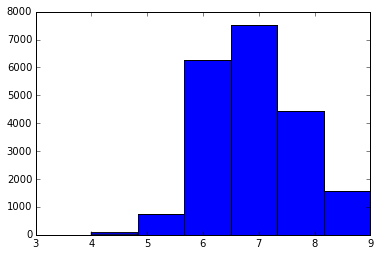
\includegraphics[height=4in]{reliability}
\end{centering}
\end{figure}




\section{Conclusions}

\bibliographystyle{abbrvnat}
\bibliography{SETs}

\end{document}
